% Software Development for Mobile Devices
\documentclass[11pt,english,numbers=endperiod,parskip=half]{scrartcl}

\usepackage{color}
\usepackage{graphicx}
\usepackage{minted}
\usepackage{fancyhdr}
\usepackage{pdflscape}
\usepackage{listings}
\usepackage{pifont}

\newcommand{\cmark}{\ding{51}}

\pagestyle{fancy}

\rhead{Daniel Parker - 971328X}
\lhead{COS30017 - Software Development for Mobile Devices}

\title{Portfolio Report}
\subtitle{COS30017 - Software Development for Mobile Devices}
\author{Daniel Parker 971328X}

\date{\today}

\begin{document}
\maketitle
\thispagestyle{empty}

\section{Overview}

\section{Evidence}
\textit{\textbf{-} = in progress}
  \begin{table}[H]
    \begin{tabular}{|l|c|}
      \hline
      Assessment & Completed \\
      \hline
      Core Assignments (for Pass) & \cmark \\
      \hline
      Extension Tasks (for Credit) & \cmark \\
      \hline
      Custom Application (for Distinction) & \textbf{-} \\
      \hline
      Research Report (for HD) & \textbf{-} \\
      \hline
    \end{tabular}
  \end{table}
  Project brief has been submitted for custom application and I also intend on
  completing the HD research report as well.
\section{Reflection}
  \subsection{Concept Map}
    \begin{figure}[H]
    \centering{
      \fbox{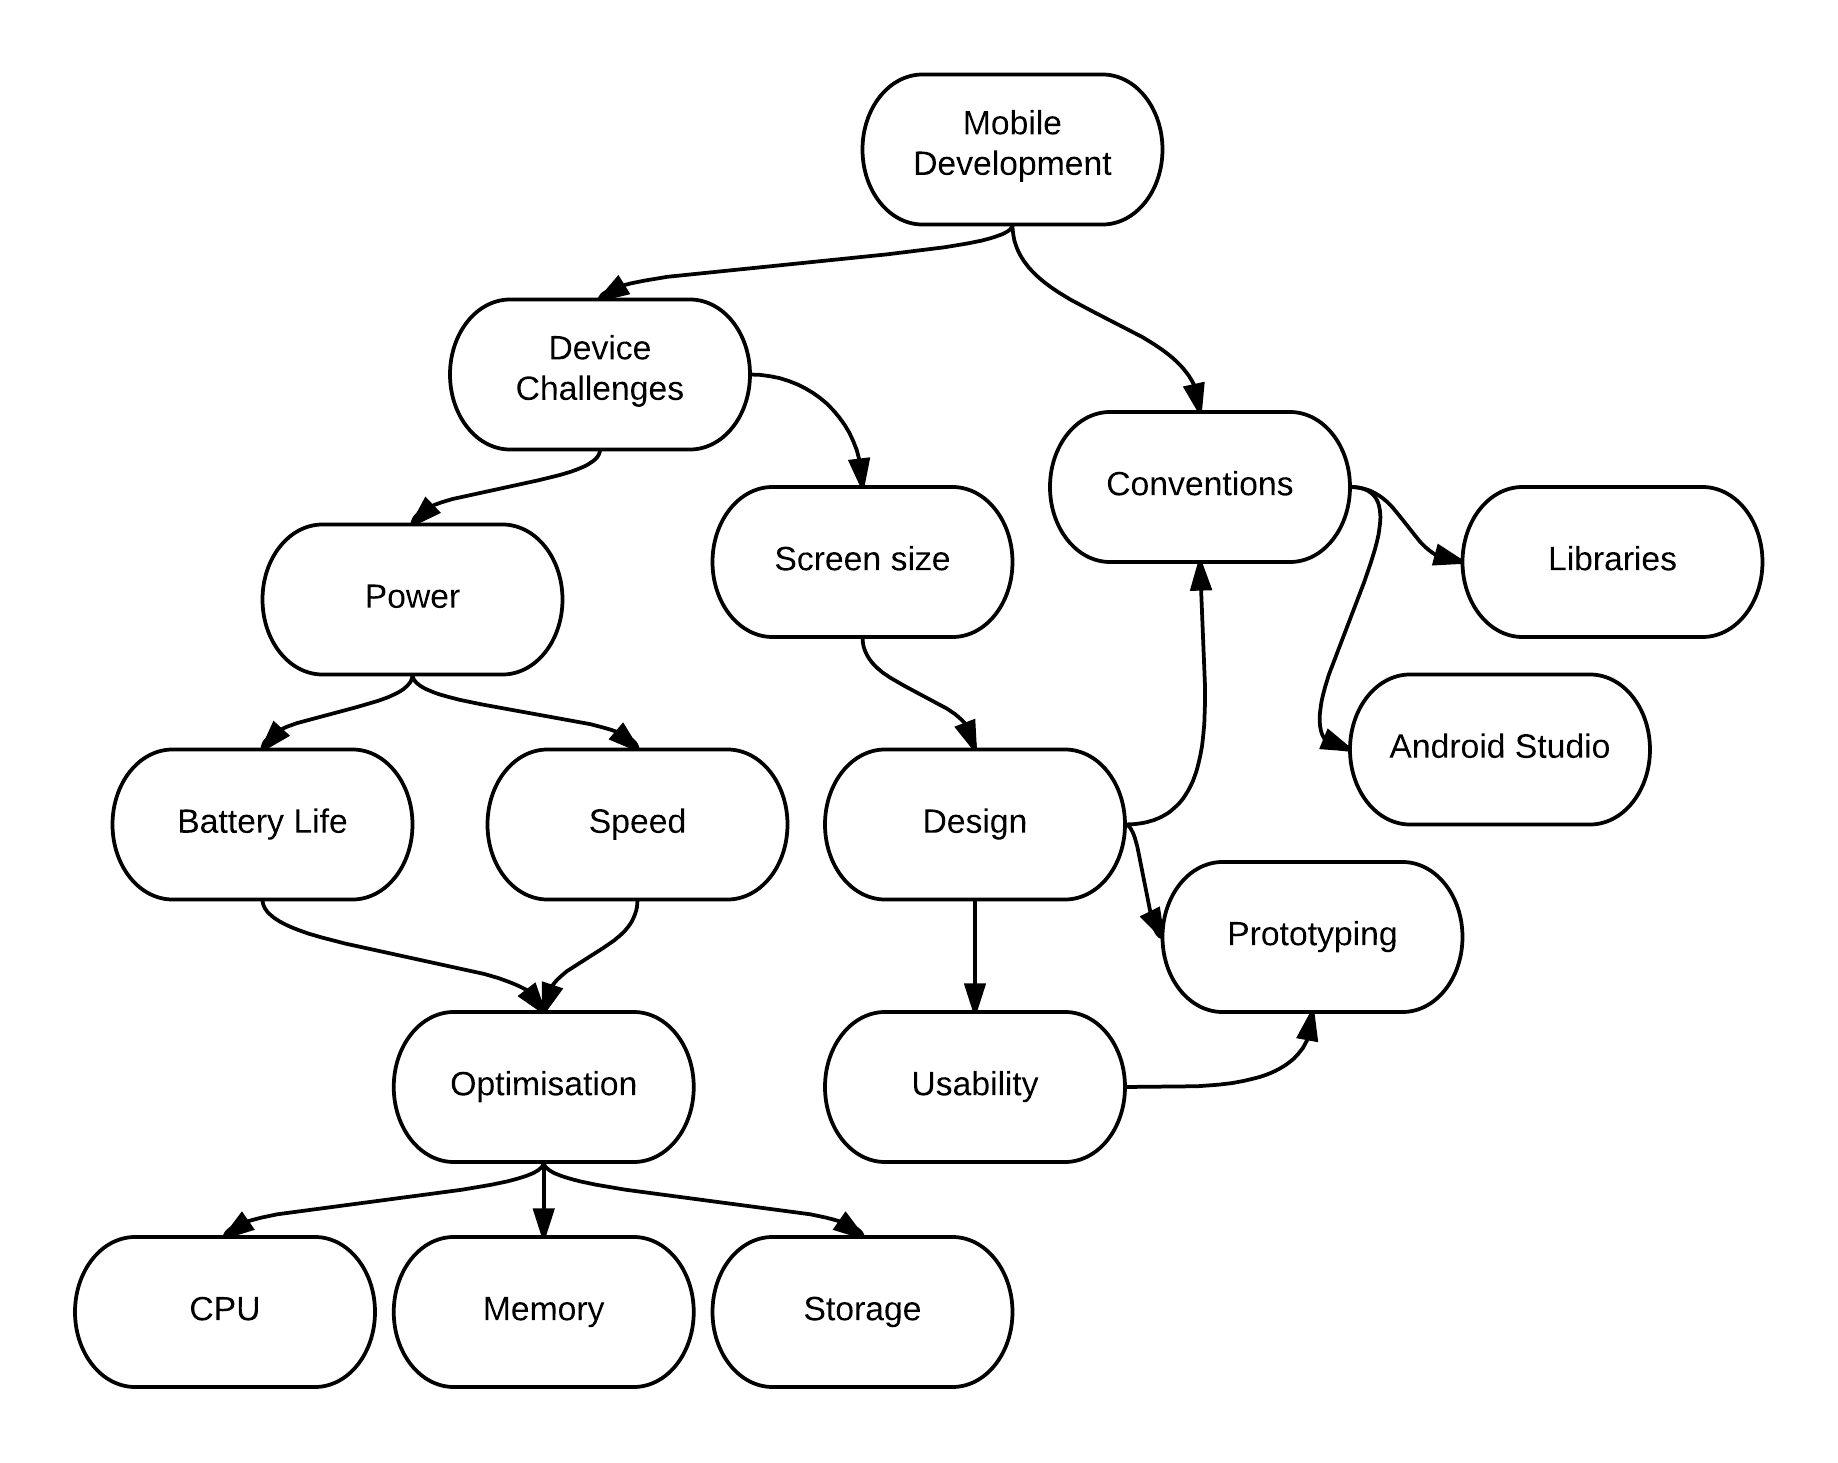
\includegraphics[width=\textwidth]{images/mind_map.png}}
    }\\
    \end{figure}
  \subsection{Mobile Application Development Process}

  \subsection{Analysis and Problem Solving Approaches}

  \subsection{Comparison and Contextual Placement}

  \subsection{Generalization}

  \subsection{Challenges in Mobile Development}

  \subsection{Explorations}

\end{document}
